\subsubsection{Konzept zur Verkettung von Effekten}
\label{sec:DSPChaining}

In einem nachfolgenden Schritt, soll die Software in der Lage sein, mehrere DSP Effekte hintereinander zu schalten. Nachfolgend ist ein Konzept beschrieben, wie die DSP Daten von Block zu Block weitergereicht werden können.

\begin{figure}[H]
	\centering
	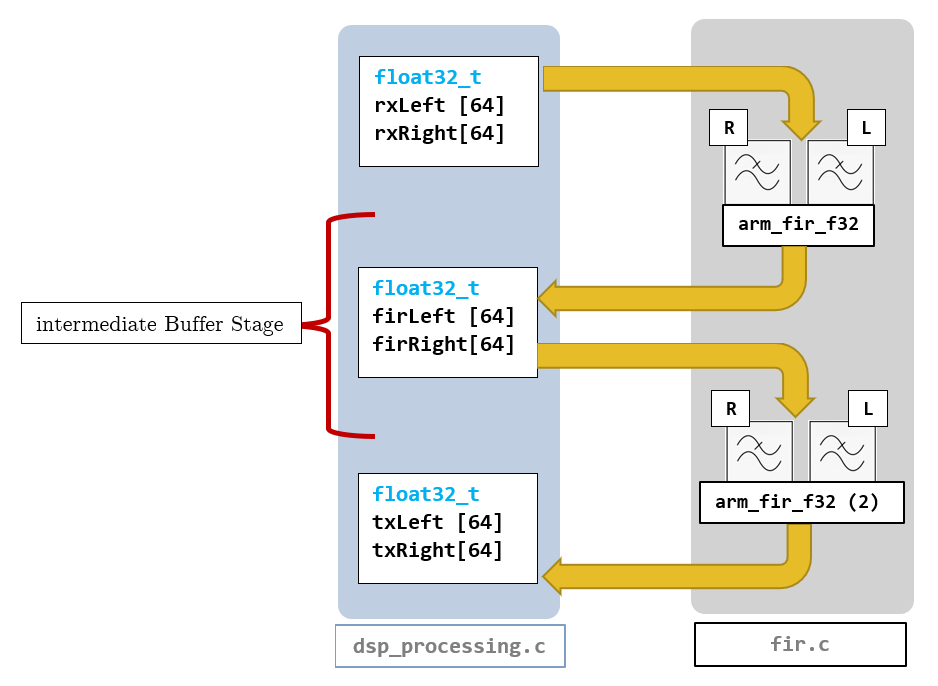
\includegraphics[width=0.8\linewidth]{Buffer_stage}
	\caption{Mögliche Erweiterung der FIR Funktion aus dem \texttt{dsp\_processing.c} durch Verwendung eines dazwischenliegenden Buffers.}
	\label{pic:Buffer_stage}
\end{figure}

Die Abbildung \ref{pic:Buffer_stage} zeigt die letzten beiden Abschnitte der Datenverarbeitung. Die Datei \texttt{fir.c} bleibt unverändert und enthält weiterhin nur FIR Filter. An ihrer Stelle könnte auch eine andere Datei mit anderen DSP Funktionen stehen.
Die Daten werden in Form eines Buffers an die nächste Funktion weitergereicht.
Damit die Datenverarbeitung wie gewünscht funktioniert, muss im \texttt{dsp\_processing.c} das Management der Buffer im Sinne von "\textit{Verbindungskabel}" verwaltet werden.

Das nachfolgende Listing zeigt das Beispiel aus Abbildung \ref{pic:Buffer_stage}, bei dem die Daten durch zwei FIR Filter durchgereicht werden.

\begin{lstlisting}[style=Cuvision, caption={Daten mittels Buffer und zwei FIR Filter bearbeiten}]
// process rxLeft in FIR(1), store in intermediate buffer: firLeft
arm_fir_f32(&FIR_F32_Struct_1, rxLeft, firLeft, blockSize);
// process firLeft in FIR(2), output to txLeft
arm_fir_f32(&FIR_F32_Struct_2, firLeft, txLeft, blockSize);

\end{lstlisting}

Dieses Konzept weist folgende drei Punkte auf, die beim Design beachtet werden müssen.
Einerseits nimmt mit jedem Buffer dazwischen die \textbf{Latenzzeit} um $t_{lat}=BUFFERSIZE*t_S=64*\frac{1}{48'000\si{Hz}}=1.3\si{ms}$ zu.
Weiterhin steigt mit der Anzahl Buffer auch der \textbf{RAM Bedarf} um $BUFFERSIZE*n_{Bytes}*n_{channels}=64*2*2=256\si{Bytes}$ pro Buffer.
Zuletzt steigt mit jedem neuen Effekt auch die \textbf{Rechenzeit}. Diese muss in jedem Fall individuell beachtet werden, da sie auch stark von der Art des Effektes abhängt.
Die gesamte Rechenzeit darf auf keinen Fall länger als die oben berechneten $1.3\si{ms}$, die der zeitlichen Länge eines Buffers beträgt, sein.

Weitere Details zum Ressourcenbedarf und Timing der DSP Funktionen sind dem Abschnitt \ref{sec:DSP_Timing} aus der Validierung zu entnehmen.

\subsubsection{Grobkonzept für das Backend der Benutzersoftware}

\begin{figure}[H]
	\centering
	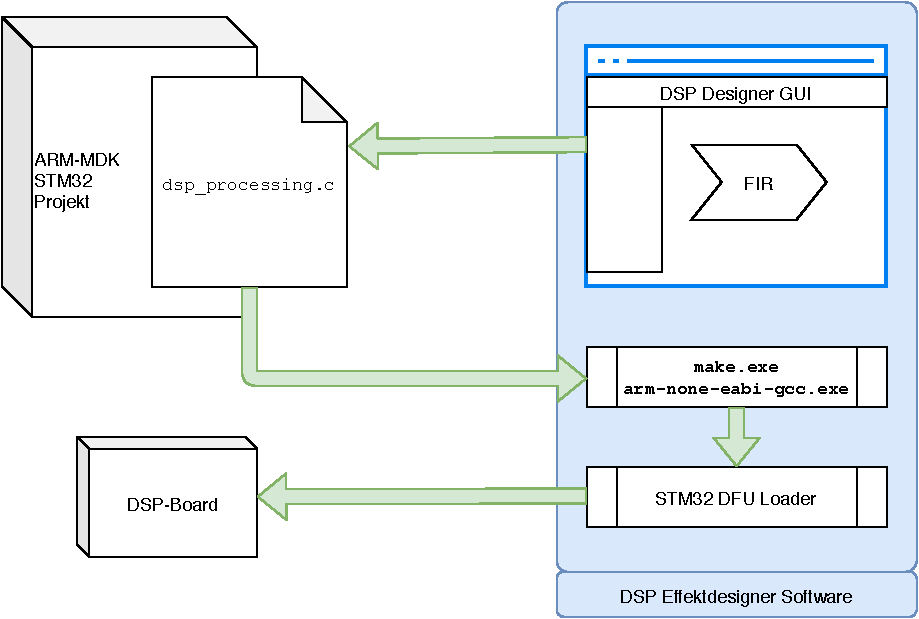
\includegraphics[width=0.8\linewidth]{arm_mdk_gui.pdf}
	\caption{Interaktion der Backend Komponenten der Benutzersoftware.}
	\label{pic:arm_mdk_gui}
\end{figure}

Die Abbildung \ref{pic:arm_mdk_gui} zeigt einen groben Überblick, wie die angedachte Benutzersoftware im Hintergrund arbeitet. 
Als Ausgangslage dient die Projektstruktur (MDK-ARM) mit der Datei für die Signalverarbeitung \texttt{dsp\_processing.c} sowie allfällige Dateien für um Bedienelemente auf Funktionen zuzuweisen.
Das Programm verändert/erstellt diese Datei und leitet das ganze Projekt an den Compiler \texttt{arm-none-eabi-gcc} resp. \texttt{make} weiter.
Bei der Erstellung der Software, muss beachtet werden, dass diese selber den Compiler mitliefern soll. 
Dabei besteht der Vorteil, dass der Compiler \texttt{arm-none-eabi-gcc} Open Source \cite{ARM-NONE-EABI} ist und beispielsweise als Package in JavaScript (über NPM) \cite{NPM-ARM} verfügbar ist.
Weiterhin werden die Funktionen von STMicroelectronics für das DFU Interface mit der STM32 MCU benötigt, um die Binaries zu konvertieren und auf das Board zu flashen.




